\chapter{Confucius}  

Versions citées : Anne CHENG (trad.), Les Entretiens de Confucius, Paris : Seuil, 1981.  Jean LEVI (trad.), Les deux arbres de la Voie : Les Entretiens de Confucius, Paris : Belles Lettres, 2018.   Pierre RYCKMANS (trad.), Les Entretiens de Confucius, Paris : Gallimard, 1987.  

\section{rappel historique - L’époque de Confucius (551-479 av. J.-C.)}

\paragraph{la dynastie des zhou}
 
les Zhou de l’Ouest ou Zhou occidentaux (1045-771 AEC).
 
 
les zhou orientaux (770-221 AEC), eux mêmes divisés en deux périodes : 
\begin{itemize}
    \item les printemps et automnes (771-481). \textit{Les annales qui relatent les événements} et \textit{le stratagèmes des royaumes combattants}
    \item les Royaumes combattants (481-221 AEC). Le roi nomme des \textit{hegemons}. 
\end{itemize}
\begin{figure}[!h]
    \centering
    \sidecaption{Géographie des Etats des Zhous Occidentaux Source: Li Feng, « The Western Zhou State », dans Paul R. Goldin (2018), p. 87}
    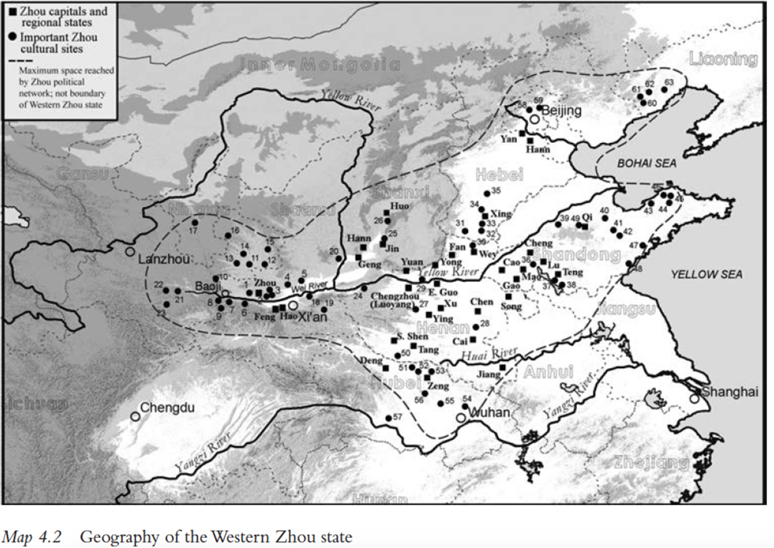
\includegraphics[width=\textwidth]{ConfucianismeTaoismeBouddhismeChinois/Images/zhouville.png}

    \label{fig:enter-label}
\end{figure}

\paragraph{Fondement politique de la dynastie Zhou:}  le système fengjian   封建 : « délimiter des frontières et établir des États ».	semblable au système féodal en Occident



\paragraph{Système des lignées } : système politico-rituel destiné à réguler la transmission des prérogatives politiques

\begin{figure}[!h]
    \centering
    \sidecaption{\textbf{Le système Tsung-fa} - source : Cho-yun Hsu, Katheryn M. Linduff, Western Chou Civilization, New Haven; London: Yale University Press, 1988, p. 164.}
    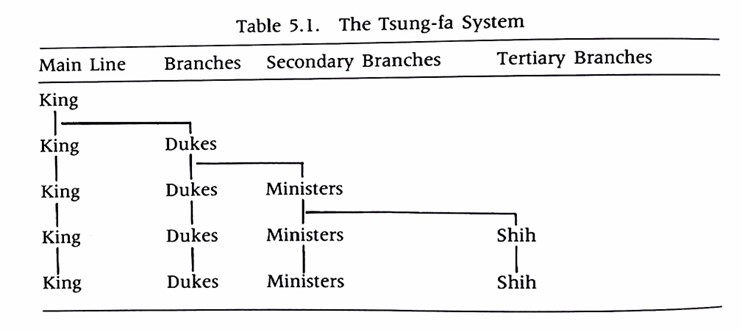
\includegraphics[width=\textwidth]{ConfucianismeTaoismeBouddhismeChinois/Images/SytemeLignee.jpg}

    \label{fig:enter-label}
\end{figure}

\begin{quote}
    Fort peu de textes
peuvent nous donner une idée de ce qu'était la civilisation antérieure à la
conquête ; toutefois, on peut considérer comme admis que le tsung-fa, le
culte des ancêtres qui intégrait les membres des clans de l'aristocratie Chou
dans une hiérarchie extrêmement rigide dont le principe est le degré de
parenté avec l'ancêtre fondateur de la dynastie, était déjà en germe dans
le système de culte des ancêtres beaucoup moins élaboré que pratiquaient
les souverains Shang. \textit{ \small Cartier Michel. Wolfram Eberhard,\href{https://www.persee.fr/doc/ahess_0395-2649_1968_num_23_5_421998_t1_1128_0000_2}{Conquerors and rulers, social forces in medieval China} .. In: Annales. Economies, sociétés,
civilisations. 23ᵉ année, N. 5, 1968. pp. 1128-1131;} 

\end{quote}
Chaque lignage est fragmenté en plusieurs branches: une branche principale et plusieurs branches mineures.


\paragraph{Le fondement religieux de la dynastie Zhou:}

Le système des temples aux ancêtres :

\begin{figure}[!h]
    \centering
    \sidecaption{Configuration du système de temple des ancêtres Zhous. Less rois Wu, Cheng,... sont des rois zhous. Source : Li Feng (2013), p. 145.}
    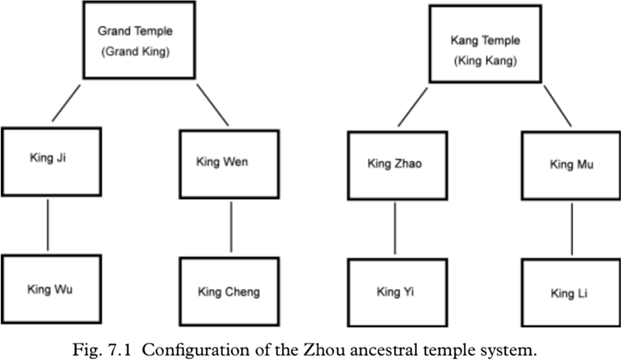
\includegraphics[width=\textwidth]{ConfucianismeTaoismeBouddhismeChinois/Images/zhoutemple.png}

    \label{fig:enter-label}
\end{figure}

Après la conquête, cette organisation en 5 temples a été dupliquée dans toutes les principales villes royales et chefs-lieux des États régionaux.
Culte commun aux élites Zhou.


\paragraph{les 5 Hégémons de La période des Printemps et automnes}  (771-481/53 AEC), première moitié de la dynastie des Zhou orientaux (770-221 AEC).

\begin{figure}[!h]
    \centering
    \sidecaption{{La période des Printemps et automnes (771-481/53 AEC), première moitié de la dynastie des Zhou orientaux (770-221 AEC).}
    \includegraphics[width=\textwidth]{ConfucianismeTaoismeBouddhismeChinois/Images/PrintempsAutomne.png}

    \label{fig:enter-label}
\end{figure}

\section{Maitre Kong}
Confucius (Kongfuzi, maître Kong, 551- 479 av. J.-C. )
\begin{marginfigure}
    \centering
    \caption{Portrait de Confucius, Ma Yuan (1160-1225).}
    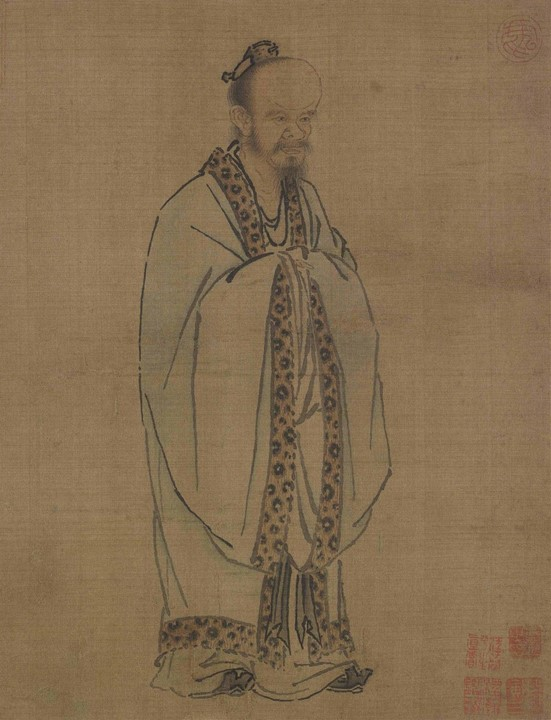
\includegraphics[width=\textwidth]{ConfucianismeTaoismeBouddhismeChinois/Images/Confucius.jpg}

    \label{fig:enter-label}
\end{marginfigure}

\paragraph{famille de petite noblesse}Né dans une famille de la petite noblesse du rang des officiers dans le pays de Lu
\paragraph{Rang d'officier de Maitre Kong} A la fois, membre de la famille royale et à la fois fonctionnaire. Son nom personnel: Qiu (Colline)
Pourquoi un nom social (zhongni - \textit{Ni} le puinê) ? Cela permet de s'adresser aux personnes car sinon, c'est malpoli.
Mais quand on parle de soi, on part de son prénom.


\paragraph{les entretiens}
\begin{itemize}
    \item  	Divisé en 20 chapitres et comportant un peu plus de 500 paragraphes, cette œuvre aurait été une compilation des notes prises du vivant du maître par chacun des disciples séparément et réunies après sa mort pour former un recueil de dialogues entre le maître et ses disciples ou ses contemporains.
    \item 	un historien du 1er siècle de notre ère (Ban Gu) mentionne trois versions de ce recueil. Preuve que ce recueil existe déjà bien avant cette date.
    \item 	Le titre de chaque chapitre est constitué par les deux premiers caractères qui ouvrent le chapitre.
\end{itemize}



\section{La personne de Confucius : }

\begin{itemize}

     \item  1. \newline Le Maître\sn{grand passion des études. indépendant : à 30 ans, il acquiert une indépendance morale : il a trouvé sa voie. \newline A 40 ans, perspicacité vis à vis du monde \newline Normalement le mandat céleste est là pour l'empereur. Ici quelque chose de très profond.  Glissement sémantique très important. \newline liberté à 60 ans. \textit{on voit une progression quand on s'attelle à l'étude. } } a dit : À quinze ans, j’avais le cœur à l’étude, à trente j’étais indépendant, à quarante je n’hésitais plus, à cinquante je connus mon lot [je connaissais les décrets du ciel, le mandat céleste], à soixante mes oreilles s’étaient faites à tout, maintenant que j’en ai soixante-dix, je lâche la bride à mes passions sans jamais dépasser la mesure.   \textit{\small -- Les Entretiens, II. 4, traduction de Jean Levi, p. 8.  } 
\item 2. \newline Le Grand Intendant s’étant étonné auprès de Zigong [disciple de Confucius] que Confucius puisse être un saint avec tous ses talents divers, celui-ci rétorqua :  -- Assurément le Ciel, tout en le destinant à la sainteté, s’est plu à le doter de toutes sortes de capacités. Ces propos étant revenus aux oreilles du Maître, celui-ci déclara :  \newline -- Me connaît-il, ce Grand Intendant ! Ayant connu la pauvreté dans ma jeunesse \sn{fils non reconnu de son père, il a du faire tous les métiers}, il m’a fallu exercer toutes sortes de petits métiers. L’homme noble a-t-il de multiples talents ? Non, il n’en a pas.  \textit{\small -- Les Entretiens, IX. 6, traduction de Jean Levi, p. 58.  }
\item 3. \newline Quelqu’un demande à Confucius : Maître, comment se fait-il que vous n’exerciez aucune fonction officielle ?  À quoi Confucius répond :  Il est dit dans le Livre des Documents : « Être bon fils, être simplement bon fils et bon frère, c’est déjà prendre part au gouvernement. » Vous voyez donc que point n’est besoin d’occuper un poste pour remplir une fonction.  \textit{\small -- Les Entretiens, II. 21, traduction d’Anne Cheng, p. 36-37.  
}
\item 4. \newline Escogriffe des Marais \sn{l'être humain est fondamentalement social et pour se perfectionner, il faut vivre dans la société, même si elle est en desordre. ON ne peut pas vivre en tant qu'ermite} et Éminence Engloutie bêchaient et labouraient de concert. Confucius envoya Zilu leur demander où se trouvait le gué. \newline -- C’est qui celui là-bas qui conduit la voiture ? demanda Escogriffe des Marais. \newline -- C’est Confucius. \newline -- Le Confucius de Lu ? \newline -- C’est ça. \newline -- Il connaît le gué.  \newline Zilu s’adressa alors à Éminence Engloutie, lequel l’apostropha :  \newline -- Toi, tu es qui ? \newline -- Je suis Zilu.\newline  -- Tu ne serais pas, par hasard, un disciple de Confucius ? \newline -- En effet.  \newline -- L’empire est pris dans un tourbillon ; qui peut rien y changer ? Pourquoi, au lieu d’être à la remorque de quelqu’un qui va de l’un à l’autre, ne suivrais-tu pas plutôt des sages qui ont su fuir le monde ? \newline  Sur ce, il se remit à bêcher sans désemparer. Zilu s’en fut rapporter ces propos au Maître. Celui-ci resta un moment perplexe avant de s’exclamer :  \newline  -- Je ne puis tout de même pas vivre en compagnie des oiseaux et des quadrupèdes ! Si je refusais de fréquenter mes semblables, dans la société de qui vivrais-je ? Et puis, il va de soi que si l’ordre régnait dans le monde je ne me mêlerais pas de vouloir le changer.  \textit{\small -- Les Entretiens, XVIII. 6, traduction de Jean Levi, p. 129-130.  }

\item 5. \newline Alors que Zilu s’apprêtait à passer la nuit au gîte de la Porte de Pierre, le gardien de l’octroi lui demanda : \newline-- D’où venez-vous ? \newline -- De chez Confucius, répondit Zilu. \newline-- Ah, fit l’homme, n’est-ce pas celui qui s’obstine dans une tâche qu’il sait impossible ?  \textit{\small -- Les Entretiens, XIV. 36, traduction de Jean Levi, p. 104.  }
\item 6. \newline Le Maître a dit : Je n’ai jamais refusé d’instruire personne pourvu qu’on se présente à moi en y mettant un minimum de forme. \textit{\small -- Les Entretiens, VII. 7, traduction de Jean Levi, p. 44.   
}
\end{itemize}
 \begin{marginfigure}
    \centering
    \caption{Zengzi posant des questions sur la piété filiale à Confucius, dynastie Song (960-1279)}
    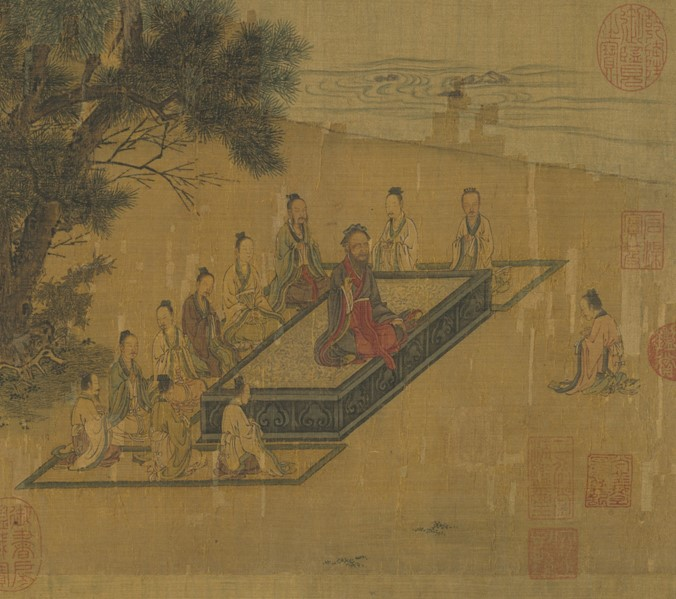
\includegraphics[width=\textwidth]{ConfucianismeTaoismeBouddhismeChinois/Images/EnseignementConfucius.jpg}

    \label{fig:enter-label}
\end{marginfigure}
\begin{Synthesis}
    vie d'errance. Il veut enseigner aux Rois et revenir à l'ordre moral du passé, sa façon d'exercer la politique. 
    Il est ouvert à tous, extraction paysanne. 
\end{Synthesis}


\paragraph{livre de poèmes } : raconte les paroles des anciens rois sages. On connait par coeur ces livres : deux personnes nobles qui se rencontrent doivent citer ces poèmes.
\paragraph{livre des mutations} livre de divination
\section{L’idéal de l’homme chez Confucius :}  
\begin{Def}[Le junzi 君子]
     (homme de bien, honnête homme, gentilhomme, homme noble)   
\end{Def}

\begin{Synthesis}
    Tous les hommes peuvent devenir des \textit{hommes de bien} par l'éducation.  "on ne nait pas noble, on le devient". 
    philosophe comme Ben Sira.
\end{Synthesis}
\begin{itemize}
    
\item 7. \newline Le Maître dit : « L’honnête homme cherche la vérité [dao : voie à emprunter], il ne cherche pas un gagne-pain. Labourez, et vous ne mangerez pas nécessairement à votre faim. Étudiez, et vous ferez peut-être carrière. L’honnête homme se soucie de la vérité, il ne se soucie pas de la pauvreté. » \textit{\small -- Les Entretiens, XV. 88, traduction de Pierre Ryckmans, p. 88. } 
\item 8. \newline Le Maître dit : L’homme de bien\sn{On n'est pas fait pour être utile à un seul métier. Mais pour lui, le sens de son existence n'est pas dans son travail. Rechercher quelque chose de plus noble. L'enseignement a plusieurs façons d'être : transmettre des connaissances ou former des personnes} n’est pas un ustensile destiné à un seul usage. \textit{\small -- Les Entretiens, II. 12, traduction d’Anne Cheng, p. 35.  }
\item 9. \newline Confucius dit \sn{dimension spirituelle : se détacher de son moi} : L’homme de bien a respect pour trois choses : les Décrets du Ciel [respect pour les choses qui dépassent l'homme], les hommes éminents et les paroles d’un Sage. L’homme de peu ne craint pas la Volonté Céleste pour la simple raison qu’il ne la connaît pas, prend des libertés avec les grands et tourne en dérision les paroles du Sage. \textit{\small -- Les Entretiens, XVI. 8, traduction d’Anne Cheng, p. 131. }
\item 10. \newline Zilu demanda ce qui constitue un gentilhomme. \newline Le Maître dit : « Il se cultive, et acquiert ainsi de la gravité. – Est-ce tout ? – Il se cultive, et donne ainsi la paix à autrui. – Est-ce tout ? – Il se cultive, et donne ainsi la paix au peuple. Mais là, Yao et Shun eux-mêmes ont peiné. \textit{\small -- Les Entretiens, XIV. 42, traduction de Pierre Ryckmans, p. 83.  }
\textit{en chinois, la gravité est le même signe que }respect.


\item 11. \newline  Sima Niu : Qu’est-ce qu’un homme de bien ? \newline Le Maître dit : L’homme de bien est celui qui n’a ni inquiétudes, ni craintes. Sima Niu : Ni inquiétudes, ni craintes—c’est donc cela l’homme de bien ? \newline Le Maître : Si, regardant en lui-même, il n’y trouve aucune tache, quelles inquiétudes, quelles craintes pourrait-il avoir ? \textit{\small -- Les Entretiens, XII. 4, traduction d’Anne Cheng, p. 96.   3 }
\item 12. \newline Le Maître voulait émigrer chez les Barbares. On lui dit : « Comment pourriez-vous vous accommoder d’une existence sauvage ? » \newline Le Maître répondit : « Là où réside l’honnête homme, il n’y a pas de sauvagerie qui tienne. » \textit{\small -- Les Entretiens, IX. 14, traduction de Pierre Ryckmans, p. 51.  }

\textit{ 
    On a une image que les barbares sont attirés par la culture chinois. Même chez les barbares, si on est honnête homme, on le reste. }
 


\item 13. \newline Le duc Ling de Wei interrogea Confucius sur l’art de manœuvrer les armées. Confucius répondit : \newline « Je sais l’une ou l’autre chose en ce qui regarde l’art de disposer les vases rituels, mais je n’ai jamais étudié celui de disposer les régiments et les bataillons. » \newline Il s’en alla le lendemain.          Au pays de Chen, on lui coupa les vivres. Ses disciples affaiblis ne tenaient plus sur leurs jambes. Indigné, Zilu vint le trouver et dit : \newline « Se peut-il qu’un honnête homme tombe dans la détresse ? » \newline Le Maître dit : « Bien sûr qu’un honnête homme peut tomber dans la détresse. Dans la détresse, seul l’homme vulgaire se laisse démonter. »  \textit{\small -- Les Entretiens, XV. 1-2, traduction de Pierre Ryckmans, p. 84.  }

 
 \textit{   Est ce que cela vaut le coup de se cultiver alors qu'on peut tomber dans la détresse. Mais l'homme de peu se laisse démonter.
    Dialogue un peu tragique. }
 
\end{itemize}
\paragraph{Le junzi par opposition au xiaoren 小人 (homme de peu, homme vulgaire)  }
\begin{Synthesis}
    Devoir vs Profit. 
    De petites choses à intérioriser. 
\end{Synthesis}
\begin{itemize}

\item 14. \newline L’homme de bien exige tout de lui-même, l’homme de peu attend tout des autres.  \textit{\small -- Les Entretiens, XV. 20, traduction d’Anne Cheng, p. 124.  }
\item 15. \newline Le Maître a dit :  L’homme noble conçoit tout en termes de devoir, l’homme vulgaire de profit. \textit{\small -- Les Entretiens, IV. 16, traduction de Jean Levi, p. 23.  }
\item 16. \newline Le Maître dit : L’homme de bien aide à s’accomplir ce que les autres ont de bon, non ce qu’ils ont de mauvais. L’homme de peu fait tout le contraire.  -- \textit{\small Les Entretiens, XII.  16, traduction d’Anne Cheng, p. 99.  }
\end{itemize}
\paragraph{Apprendre (xue 學) pour s’accomplir   }
\begin{itemize}
    
\item 17. \newline Le Maître dit \sn{l'amour de confucius a pour l'apprentissage. Il faut aimer les choses. Apprendre, il faut engager son vécu, sa personne, éprouver la joie pour les études.} : « N’est-ce pas une joie d’étudier, puis, le moment venu, de mettre en pratique ce que l’on a appris ? N’est-ce pas un bonheur d’avoir des amis qui viennent de loin ? Et n’est-il pas un honnête homme celui qui, ignoré du monde, n’en conçoit nul dépit ? » -- \textit{\small Les Entretiens, I. 1, traduction de Pierre Ryckmans, p. 13.  }
\item 18. \newline Le Maître dit : « Autrefois on étudiait pour soi, \sn{dans la dynastie des Song où le bouddhisme arrive, on s'interroge sur le \textit{soi}, lien entre \textit{connaissance} et \textit{soi}, quand assimiler les connaissances ? } aujourd’hui on étudie pour impressionner les autres. » -- \textit{\small Les Entretiens, XIV. 24, traduction de Pierre Ryckmans, p. 80.  }
\item 19. Fan Chi prie  le Maître de lui enseigner l’agriculture. \newline Le Maître : Pour cela, adresse-toi plutôt à un vieux paysan. Fan Chi lui demande alors des instructions sur le jardinage. \newline Le Maître : Pour cela, tu ferais mieux d’aller voir un vieux jardinier.    \newline     Le disciple sorti,  le Maître s’exclame : Un homme de bien peu, ce Fan Chi ! Que les gouvernants s’attachent au rituel, et il ne se trouvera personne dans le peuple pour y contrevenir ; qu’ils s’attachent au Juste, et il n’y aura pas un signe d’insoumission ; qu’ils s’attachent à la bonne foi, et personne n’osera parler contre la vérité. C’est ainsi qu’ils verront venir à eux de toutes parts le peuple entier, les mères accourant avec leurs enfants sur le dos. Que leur servirait de savoir cultiver la terre ? \textit{\small -- Les Entretiens, XIII. 4, traduction d’Anne Cheng, p. 103.    4 }

\item 20. \newline Le Maître dit : « Zigong, crois-tu que je sois quelqu’un qui étudie une masse de choses et qui les retient par cœur ? » \newline L’autre répondit : « En effet. N’en est-il pas ainsi ? \newline –Nullement. J’ai un seul fil pour enfiler le tout. » \textit{\small -- Les Entretiens, XV. 3, traduction de Pierre Ryckmans, p. 84.  }
\item 21. \newline Le Maître dit : Étudier sans réfléchir est vain ; méditer sans étudier est périlleux. -- \textit{\small Les Entretiens, II. 15, traduction d’Anne Cheng, p. 35.   }
\end{itemize}

\subsection{Les cinq vertus   le ren 仁 (le sens de l’humain)  }


\begin{itemize}

\item 22. \newline Fan Chi : Qu’est-ce que le ren ?  \newline Le Maître : C’est aimer les hommes.  […]  \textit{\small -- Les Entretiens, XII. 22, traduction d’Anne Cheng, p. 101.  }

\textit{Traduction par Anne Cheng de  ren. \textit{sens de l' humain}
}. Arriver à une véritable compassion pour les autres : aimer les hommes, en s'oubliant. Enlever toutes les frontières avec les autres. Pas très facile à mettre en pratique dans le quotidien.



\item 23. \newline Zigong demanda : « Que penseriez-vous d’un homme qui comblerait le peuple de bienfaits et qui viendrait en aide à la multitude ? Peut-on dire qu’il aurait atteint la vertu suprême ? \newline Le Maître dit : « Ceci n’a rien à voir avec la vertu suprême. Pareil homme serait un saint—même Yao et Shun seraient bien en peine de l’égaler. En revanche, pour ce qui est d’atteindre la vertu suprême, la recette est à la portée de la main : prenez pour guide vos propres aspirations—assurez à votre prochain le sort que vous vous souhaiteriez à vous-même, obtenez pour lui ce que vous souhaiteriez obtenir pour vous-même. -- \textit{\small Les Entretiens, VI. 30, traduction de Pierre Ryckmans, p. 38. } 

\textit{Pour Confucius, c'est à la portée de la main.  Des choses très concretes. Commentaire du professeur : histoire d'un moine tibetain qui après un échec amoureux, dit se consacrer à l'amour de tous. Son maître lui dit : mais si tu n'arrives pas à aimer une personne, comment aimer la multitude ? 

L'étude inclut la théorie mais aussi l'habitude. }

\item 24. \newline Qu’est-ce que le ren ? Yan Hui pose la question au Maître, qui lui répond : \newline L’homme de ren est celui qui fait effort sur lui-même pour revenir au rituel ; quiconque s’en montrerait capable, ne serait-ce qu’une journée, verrait le peuple entier honorer son ren. N’est-ce pas de soi-même, et non des autres, qu’il faut en attendre l’accomplissement ? \newline Yan Hui : Pourriez-vous m’indiquer la démarche à suivre ? \newline Le Maître : Ce qui est contraire au rituel, ne le regarde pas, ne l’écoute pas ; ce qui est contraire au rituel, n’en parle pas et, à plus forte raison, n’y commets pas tes actions. Yan Hui : Je ne suis guère intelligent, mais je ferai de mon mieux pour appliquer ce précepte. \textit{\small -- Les Entretiens, XII. 1, traduction d’Anne Cheng, p. 95.  }
\item 25.\newline Fan Chi interrogea le Maître sur la vertu suprême. \newline Le Maître dit : « Être digne dans la vie privée ; diligent dans la vie publique ; loyal dans les relations humaines. Ne pas départir de cette attitude, même parmi les barbares. » \textit{\small -- Les Entretiens, XIII. 19, traduction de Pierre Ryckmans, p. 74.  }
\paragraph{Le yi 義 (le sens du juste)}  
\item 26. \newline Le Maître dit : Dans les affaires du monde, l’homme de bien n’a pas une attitude rigide de refus ou d’acceptation. Le Juste est sa règle. \textit{\small -- Les Entretiens, IV. 10, traduction d’Anne Cheng, p. 45. } 

\paragraph{Le li 禮 (le rituel)}   

\item 27. \newline Le Maître dit : « Une politesse qui n’est pas tempérée par le rituel est fastidieuse ; une prudence qui n’est pas tempérée par le rituel est peureuse ; une bravoure qui n’est pas tempérée par le rituel est violente ; une franchise qui n’est pas tempérée par le rituel est blessante. […] » \textit{\small -- Les Entretiens, VIII. 2, traduction de Pierre Ryckmans, p. 45.  }

\textit{peut nous paraître loin du fait de l'importance des rites chez les Zhou. Mais rite : pas uniquement des pratiques. Les rites, ce sont surtout des sacrifices à offrir aux puissances. Entrer en communication avec les esprits. Tout ce qu'on offre en sacrifice nous permet d'entrer en relation avec les puissances. Etat d'esprit : ce qui est essentiel. Donc, lors des rites, il y aune tension morale sollicitée : respect. Transposition de cet esprit rituel dans la vie quotidienne. "comportes toi comme s'il y avait un invité de marque. }

\textit{tension morale : on ne fait pas les choses qui outrepasse les bonnes mesures}

\textit{l'esprit rituel,c 'est comme une ascèse pour éviter l'égo-centrisme}.

\item 28. \newline Le Maître dit : « Avec les lettres pour s’ouvrir l’esprit et
les rites pour discipliner, on ne saurait s’écarter du droit chemin. » -- \textit{\small  Les Entretiens, XII. 15, traduction de Pierre Ryckmans, p. 68.  }
\item 29. \newline Le Maître dit : « Ils disent : "les rites par-ci, les rites par-là", comme s’il s’agissait seulement d’ornement de jade et de soie ! Ils disent : "la musique par-ci, la musique par-là, comme s’il s’agissait de cloches et de tambours ! » \textit{\small -- Les Entretiens, XVII. 11, traduction de Pierre Ryckmans, p. 96.  }

\textit{il ne faut pas s'attacher uniquement aux formes mais comprendre l'esprit. Cela  nous permet d'agir de façon adéquate dans toues les situations. }
\item 30. \newline Le Maître dit : Gouvernez à force de lois, maintenez l’ordre à coups de châtiments, le peuple se contentera d’obtempérer, sans éprouver la moindre honte. Gouvernez par la Vertu, harmonisez par les rites, le peuple non seulement connaîtra la honte, mais de lui-même tendra vers le Bien.  -- \textit{\small  Les Entretiens, II. 3, traduction d’Anne Cheng, p. 33.  }


\paragraph{Le zhi 知/智 (Le discernement, la perspicacité)  }
\item 31. \newline Le Maître dit : Le sage est franc de toute incertitude, l’homme de ren de toute inquiétude, le brave de toute crainte.  \textit{\small -- Les Entretiens, IX. 28, traduction d’Anne Cheng, p. 80.  }
\item 32. \newline Le Maître dit : « L’homme sage aime l’eau, l’homme bon aime la montagne. L’homme sage est actif, l’homme bon est tranquille. L’homme sage est joyeux, l’homme bon vit longtemps. » -- Les Entretiens, VI. 23, traduction de Pierre Ryckmans, p. 37.  
\item 33. \newline Le Maître a dit : -- Zilu, veux-tu que je te dise ce que c’est que savoir ? Savoir que l’on sait quand on sait, et l’on ne sait pas quand on ne sait pas, voilà savoir.  -- Les Entretiens, II. 17, traduction de Jean Levi, p. 10.  

\textit{pour corriger ses fautes, il faut être honnête à soi même.}
\item 34. Maître Zeng dit : Chaque jour je m’examine plusieurs fois : me suis-je fidèlement acquitté de mes engagements ? Me suis-je montré digne de la confiance de mes amis ? Ai-je mis en pratique ce qu’on m’a enseigné ? \textit{\small -- Les Entretiens, I. 4, traduction de Pierre Ryckmans, p. 13.  }

\textit{Zeng, disciple de confucius mais représente la pensée de confucius. Examen de conscience permet de consolider tout ce que l'on a appris. Toujours l'idée de s'améliorer constamment. Plus d'inquiétude : si on a bien fait ce que l'on doit faire, alors le reste ne dépend pas de nous. }

35. \newline Le Maître dit : Ne crains point de rester méconnu des hommes, mais bien plutôt de les méconnaître toi-même. \textit{\small -- Les Entretiens, I. 16, traduction d’Anne Cheng, p. 32.  }

\textit{ne pas craindre le manque de réputation mais de ne pas connaître les autres}


\item 36. (Voir aussi la citation n° 17)  \newline Fan Chi : Qu’est-ce que le ren ?  \newline Le Maître : C’est aimer les hommes. \newline Fan Chi : Et la sagesse ?  \newline Le Maître : C’est connaître les hommes. (Voyant Fan Chi perplexe) C’est savoir choisir les hommes droits et les placer au-dessus des hommes pernicieux afin que ces derniers s’en trouvent redressés.  \newline 6 Fan Chi, en quittant  le Maître, rencontre Zixia : Je viens de voir  le Maître et de l’interroger sur la sagesse. Il m’a répondu : C’est savoir choisir les hommes droits et les placer au-dessus des hommes pernicieux afin que ces derniers s’en trouvent redressés. Qu’en penses-tu ? \newline Zixia : Quelle richesse dans ces quelques mots ! Lorsque Shun, devenu maître du monde, distingua Gao Yao de la multitude en l’élevant au rang de ministre, les hommes privés de ren s’éloignèrent. Lorsque Cheng Tang, devenu maître du monde, distingua Yi Yin en l’élevant au rang de ministre, les hommes privés de ren disparurent.   \textit{\small -- Les Entretiens, XII. 22, traduction d’Anne Cheng, p. 101.  } 

\textit{on voit pourquoi il faut connaître les autres. le xu, dans le gouvernement : sagesse. Savoir s'entourer des personnes compétentes et vertueuses. }
\end{itemize}

\begin{Prop}
    Importance très forte du choix des ministres : compétent ou vertueux. La base du gouvernement, c'est \textit{bien connaître les hommes} (Xu)
\end{Prop}



\paragraph{Le xin 信 (fidélité à la parole donnée, fiabilité, sincérité, confiance)}  
\begin{itemize}
     
\item 37. \newline Le Maître dit : La honte de l’homme de bien, c’est de voir ses paroles excéder ses actions. \textit{\small  -- Les Entretiens, XIV. 29, traduction d’Anne Cheng, p. 116.  }
\item 38. \newline Le Maître dit : « Mine débonnaire et belles paroles » sont rarement signe de vraie vertu.  \textit{\small -- Les Entretiens, I. 4, traduction de Pierre Ryckmans, p. 13.  }
\item 39. \newline Zizhang demanda comment agir. \newline Le Maître dit : « Parlez avec loyauté et bonne foi, agissez avec honnêteté et prudence, et votre action sera efficace, même parmi les Barbares. Si vous parlez sans loyauté ni bonne foi, si vous agissez sans honnêteté ni prudence, comment votre action pourrait-elle être efficace, même dans votre propre village ? Gardez cette maxime constamment devant les yeux, gravez-la sur le timon de votre char, et votre action sera efficace. » \newline Zizhang l’inscrivit sur sa ceinture.  \textit{\small -- Les Entretiens, XV. 6, traduction de Pierre Ryckmans, p. 85.  }


\item 40. \newline Zigong : Qu’est-ce que gouverner ? \newline Le Maître : C’est veiller à ce que le peuple ait assez de vivres, assez d’armes, et s’assurer sa confiance. \newline Zigong : Et s’il fallait se passer d’une de ces trois choses, laquelle serait-ce ? \newline Le Maître : Les armes. \newline Zigong : Et des deux autres, laquelle serait-ce ? \newline Le Maître : Les vivres. De tout temps, les hommes sont sujets à la mort. Mais sans la confiance du peuple, aucun État ne saurait tenir. -- Les Entretiens, XII. 7, traduction d’Anne Cheng, p. 97.  

\textit{solidarité dans toute la population et entre le peuple et le souverain. Pour bien fonctionner, il faut quelque chose qui relie sur le plan moral tous les individus. C'est encore plus puissant que les armées. A noter : c'est ce qu'on a vu en Ukraine. }

\item 41. \newline Zixia dit : « Un gentilhomme fait d’abord régner la confiance et ensuite il peut mobiliser ses gens. Sans cette confiance, ceux-ci pourraient se croire brimés. Un gentilhomme fait d’abord régner la confiance, et ensuite il peut critiquer son souverain. Sans cette confiance, celui-ci pourrait se croire insulté. » \textit{\small -- Les Entretiens, XIX. 10, traduction de Pierre Ryckmans, p. 105. }

 
\end{itemize}

\subsection{mort et postérité de confucius}
\paragraph{5 principales branches}
Il aurait eu trois mille disciples. Huit principales branches scolastiques  seraient apparues dont les plus éminentes furent celle de Mencius (env. 380-289) et celle de Xunzi (1ère moitié du IIIe siècle av. J.-C.).

\begin{figure}[!h]
    \centering
    \sidecaption{Portrait des disciples de Confucius, 7e siècle}
    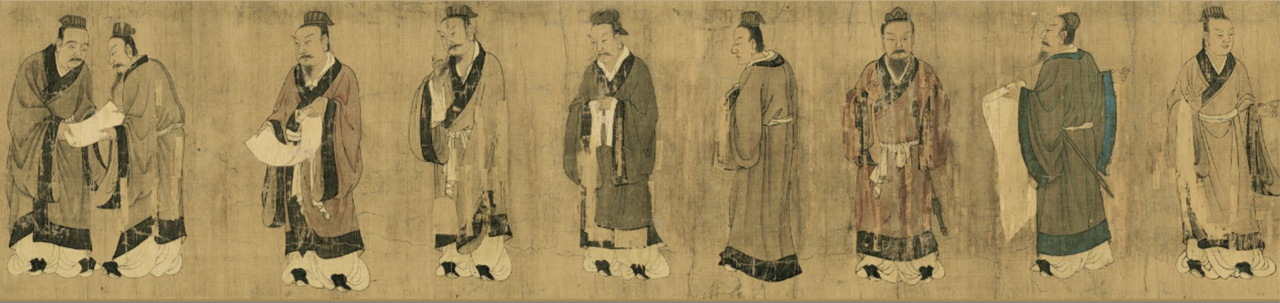
\includegraphics[width=\textwidth]{ConfucianismeTaoismeBouddhismeChinois/Images/disciplesConfucius.png}

    \label{fig:enter-label}
\end{figure}

\paragraph{Temple de Confucius}
\begin{itemize}
    \item  Des cultes du Maître ont été pratiqués dès la mort de celui-ci dans son pays natal.
  \item 	Au IIème siècle avant notre ère (début de la dynastie Han), le confucianisme devint la doctrine officielle de l’État.
  \item À partir du 4e siècle, des temples de Confucius subventionnés par l’État furent érigés dans les capitales des différentes dynasties.
  \item Au 8e siècle, Confucius se vit accorder le titre de Wenxuan wang (Roi de la propagation des lettres) par un empereur de la dynastie Tang.

\end{itemize}
\begin{Ex}[temple de Confucius]


    \begin{figure}[!h]
    \centering
    \sidecaption{Temple de Confucius dans la ville de Qufu de la province du Shandong}
    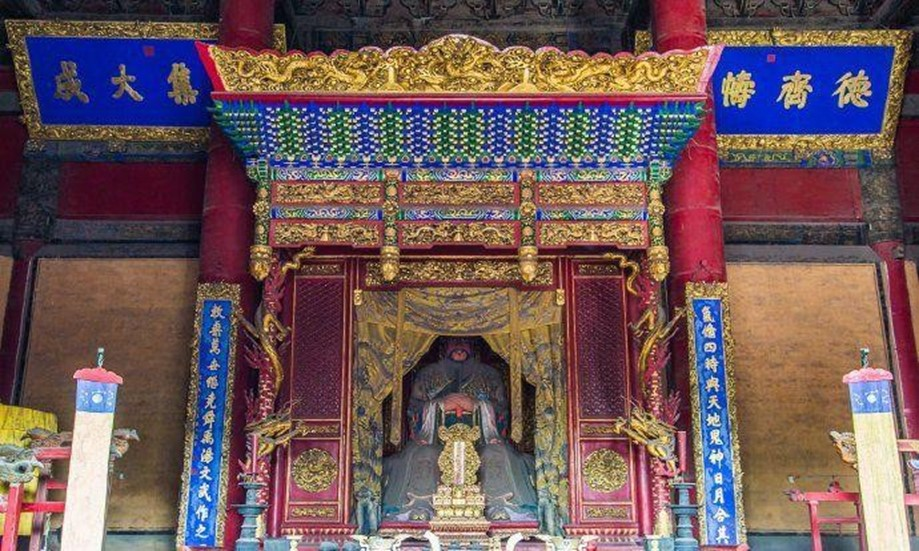
\includegraphics[width=0.8\textwidth]{ConfucianismeTaoismeBouddhismeChinois/Images/TempleConfucius.jpg}

    \label{fig:enter-label}
\end{figure}
    On voit des statues. Mais en fait, influence bouddhique fait qu'on trouve des statues dans les temples confucéens.
\end{Ex}
\paragraph{retour du confucianisme} confusion en Chine : après le développement économique, question du sens. Le choc de la pensée occidentale. Trouver une place pour la culture propre. 


\begin{Synthesis}
    A transformé l'enseignement des nobles en une morale pour tous.
\end{Synthesis}